% ============================================================
%  IEEE Conference Paper — ST-GNN for Fault Localization
% ============================================================
\documentclass[conference]{IEEEtran}

\usepackage[T1]{fontenc}
\usepackage[utf8]{inputenc}
\usepackage{amsmath,amssymb,bm}
\usepackage{graphicx}
\graphicspath{{data/}}
\usepackage{booktabs}
\usepackage{multirow}
\usepackage{hyperref}
\usepackage{cite}
\usepackage{microtype}
\usepackage[caption=false,font=footnotesize]{subfig}

\hypersetup{
    colorlinks=true,
    linkcolor=blue,
    citecolor=blue,
    urlcolor=blue,
    pdftitle={Spatiotemporal GNN for Real-Time Fault Localization in Smart Grids},
    pdfauthor={Anik Kumar Basu, Sabrina Shonda Snaha, Md. Sadik Mahmud Adive},
}

% ============================================================
\begin{document}

% ── Title ────────────────────────────────────────────────────
\title{Spatiotemporal GNNs for Real-Time Fault Localization in Power Grids}

\author{\IEEEauthorblockN{Anik Kumar Basu, Sabrina Shonda Snaha, Md. Sadik Mahmud Adive}
\IEEEauthorblockA{Department of Computer Science and Engineering\\Bangladesh University of Business and Technology, Bangladesh}}

\maketitle

% ── Abstract ─────────────────────────────────────────────────
\begin{abstract}
Fast fault detection and bus-level localization are essential for resilient
power grids under renewable integration and rapidly changing operating conditions.
Many conventional relays and topology-agnostic classifiers struggle to capture how
disturbances propagate through the network. This work presents a
\emph{Spatiotemporal Graph Neural Network} (ST-GNN) that combines spatial message passing
on the grid graph with temporal sequence modeling of PMU windows. The model uses two
Graph Convolutional Network (GCN) layers followed by a two-layer Long Short-Term Memory
(LSTM) module, trained with a multi-task objective for fault-bus localization and
fault-type classification. Experiments on the IEEE 39-bus New England system with a
synthetic dataset of $\sim$60\,000 samples (four fault types, four fault resistances, and
three load levels) achieve \textbf{92.8\%} top-1 localization accuracy, \textbf{97.4\%} fault
detection accuracy, and \textbf{1.3 buses} mean absolute bus error, outperforming classical
thresholding and standard ML baselines. Ablations indicate that both the spatial (GCN)
and temporal (LSTM) components contribute materially to performance.
\end{abstract}

\begin{IEEEkeywords}
Graph Neural Networks, Smart Grid, Fault Localization, Spatiotemporal Learning,
LSTM, GCN, Power Systems, Fault Detection, IEEE 39-Bus, Multi-Task Learning
\end{IEEEkeywords}

% ============================================================
\section{Introduction}
\label{sec:intro}
% ============================================================
Modern transmission grids are increasingly dynamic due to renewable integration,
bidirectional power flows, and high-rate sensing (e.g., PMUs) \cite{liao2021}. Faults can
propagate quickly through electrically coupled regions, so the operational goal extends
beyond detection to identifying the originating bus with low latency.

Impedance- and threshold-based relays remain useful but can degrade when parameters
shift or transients are complex \cite{chen2020}. Topology-agnostic learning (e.g., CNNs on
ordered bus vectors) can perform well in fixed settings but is not naturally
permutation-consistent with the grid graph \cite{owerko2020}. GNNs match the topology by
propagating along edges \cite{kipf2017}, but spatial-only models do not explicitly capture
the transient evolution that distinguishes fault types and severity \cite{yu2018}.

We propose a \textbf{Spatiotemporal Graph Neural Network (ST-GNN)} that couples GCN-based
spatial aggregation with LSTM-based temporal modeling over sliding PMU windows. The
main contributions are:

\begin{itemize}
  \item A hybrid GCN + LSTM architecture that jointly models graph topology and
        temporal fault dynamics on the IEEE 39-bus New England system.
  \item A synthetic dataset of $\sim$60\,000 labeled samples generated with
        Pandapower, spanning four fault types, four fault resistances (0–20\,$\Omega$),
        and three load levels (60\%–130\% nominal).
  \item A multi-task training objective that simultaneously optimizes fault-bus
        localization (primary) and fault-type classification (auxiliary), improving
        generalization of the shared backbone.
  \item Ablation and robustness studies (noise and N-1 contingencies) that quantify
    sensitivity to measurement noise and topology perturbations.
\end{itemize}

% ============================================================
\section{Related Work}
\label{sec:related}
% ============================================================

\subsection{Traditional and Shallow Learning Methods}
Traditional fault-detection pipelines relied on impedance relays, threshold rules, and
related signal-processing logic. These methods are fast and interpretable, but their
accuracy depends on accurate line parameters, relay settings, and stable operating
assumptions. In renewable-rich grids, those assumptions are less reliable because inverter
behavior, topology changes, and bidirectional power flow can alter fault signatures. Liao
et al. \cite{liao2021} and Chen et al. \cite{chen2020} both note that data-driven fault
diagnosis becomes attractive when fixed rules are no longer flexible enough.

As PMU data became more available, shallow classifiers such as SVMs, random forests,
decision trees, and shallow ANNs were adopted for fault-type classification and coarse
localization. These models can learn nonlinear boundaries, but they still depend heavily on
handcrafted features and often ignore the physical topology of the grid. For bus-level fault
localization, that limitation is serious because electrically close buses may appear unrelated
in a plain feature vector.

\subsection{Deep Learning for Fault Diagnosis}
CNN-based approaches reduce feature engineering by learning directly from waveform or
feature-map inputs, but they still assume an ordered Euclidean layout and can be sensitive
to bus indexing \cite{owerko2020}. Recurrent models, especially LSTMs, capture temporal
evolution effectively \cite{hochreiter1997}, which makes them useful for fault transients.
However, a pure temporal model does not explicitly represent electrical connectivity, so it
can miss the spatial relationships needed for bus-level localization.

\subsection{Graph Neural Networks in Power Systems}
GNNs address this mismatch by learning directly on the bus-line graph. Kipf and Welling
\cite{kipf2017} provided the graph-convolutional foundation used in many later power-system
studies. Chen et al. \cite{chen2020}, Donon et al. \cite{donon2019}, and James et al.
\cite{james2020} showed that topology-aware learning improves diagnosis and localization
performance in power networks. These results suggest that the grid topology itself should
be part of the model, not just the input feature set.

The advantage of GNNs is physical consistency. If the graph representation is constructed
correctly, the model learns from electrical neighborhoods instead of relying on arbitrary bus
indexing. GNNs also scale well for sparse networks, since real power grids have far fewer
lines than all possible bus-to-bus connections. The main limitation is that many GNN-based
approaches still use static snapshots, which may not capture enough information to
distinguish the true fault location when neighboring buses experience similar disturbances.

\subsection{Spatiotemporal Learning and Research Gap}
Spatiotemporal graph models combine graph-based spatial aggregation with temporal
sequence modeling. Yu et al. \cite{yu2018} demonstrated this idea in sequence prediction by
learning both network structure and temporal dynamics. For fault localization, the same
principle is especially relevant because the most discriminative evidence often appears in
the first few cycles after fault inception.

Still, many existing studies remain snapshot-based or focus on classification rather than
bus-level localization. Robustness under measurement noise, topology changes, and class
imbalance is also reported inconsistently. These gaps motivate the ST-GNN design used in
this paper, which combines graph message passing with temporal modeling for joint fault
location and fault-type prediction.

% ============================================================
\section{System Model and Problem Formulation}
\label{sec:model}
% ============================================================

\subsection{Power Grid as a Weighted Graph}
The IEEE 39-bus New England test system is modeled as an undirected weighted graph
$\mathcal{G} = (\mathcal{V}, \mathcal{E}, \mathbf{X}, \mathbf{W})$, where
$\mathcal{V} = \{v_1, \ldots, v_{39}\}$ is the node set (buses and substations),
$\mathcal{E} \subseteq \mathcal{V} \times \mathcal{V}$ is the edge set (46 transmission
lines and transformers), $\mathbf{X} \in \mathbb{R}^{39 \times F}$ is the node feature
matrix, and $\mathbf{W} \in \mathbb{R}^{39 \times 39}$ is the weighted adjacency matrix.
The system comprises 10 generators, 19 load buses, and 10 transit buses.

\begin{figure}[t]
  \centering
  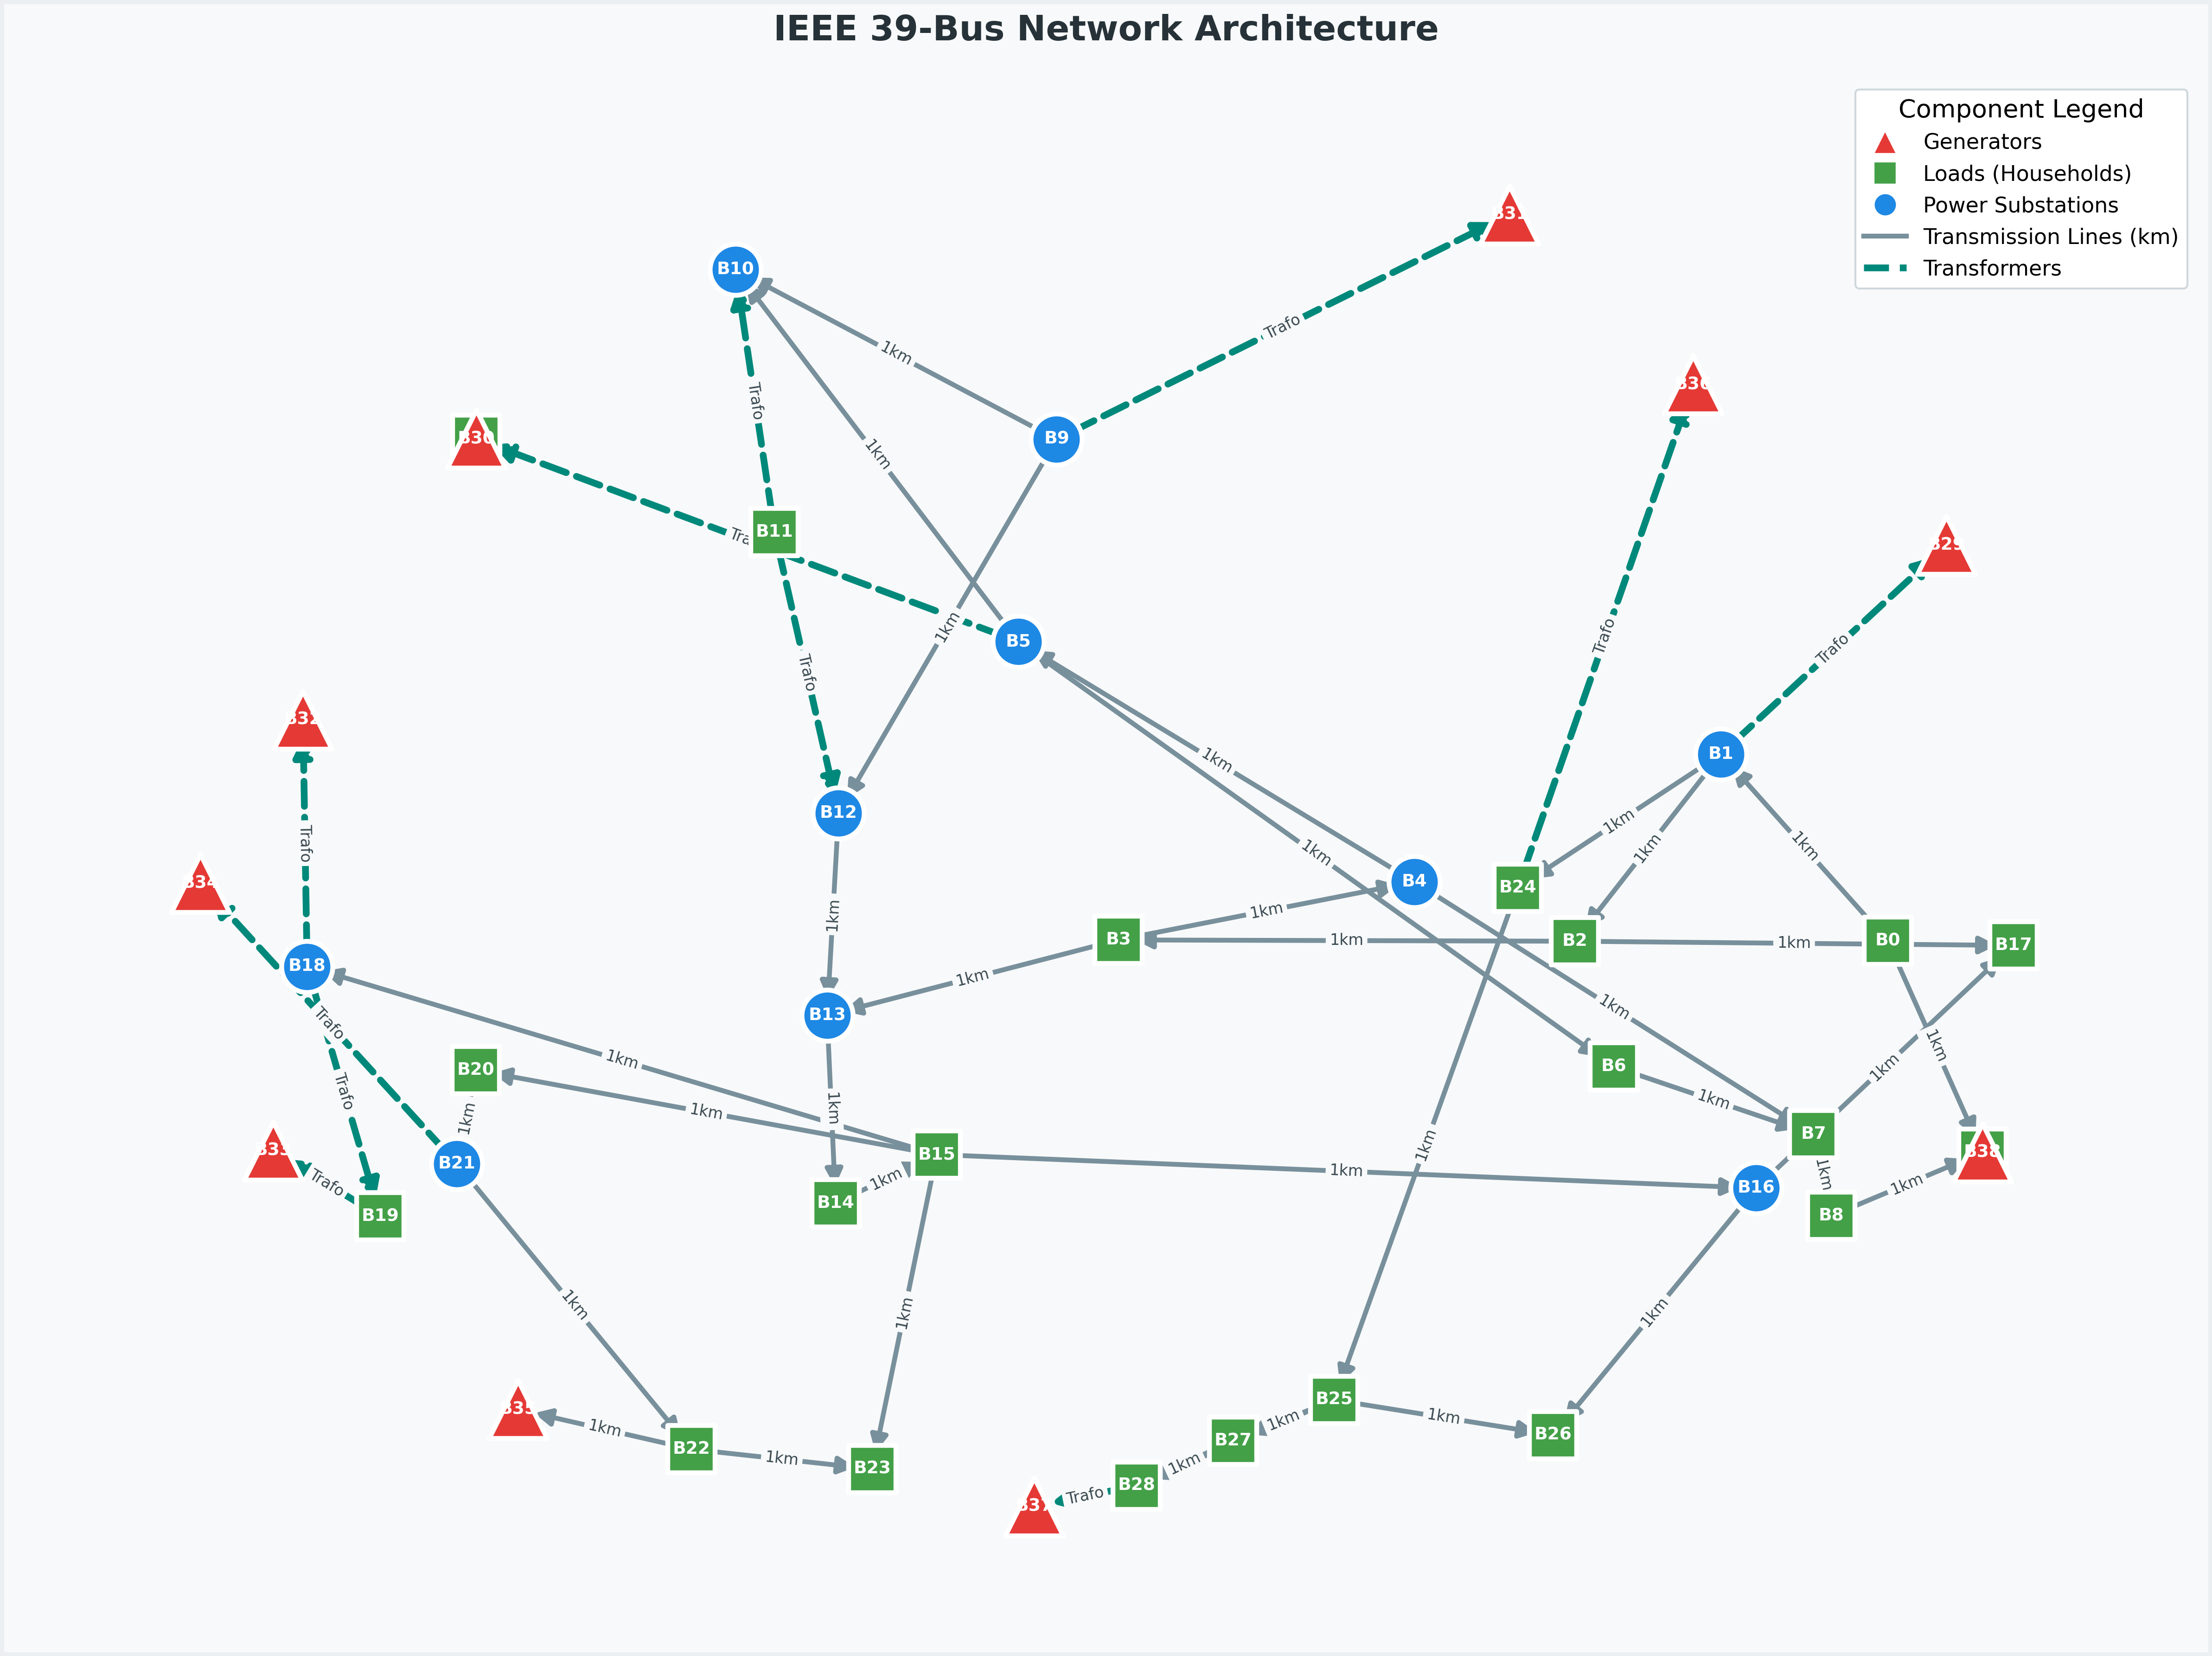
\includegraphics[width=\columnwidth]{graph_topology_clean.png}
  \caption{IEEE 39-bus topology used for message passing.}
  \label{fig:topology}
\end{figure}

\begin{figure}[t]
  \centering
  \subfloat[Binary Adjacency]{%
    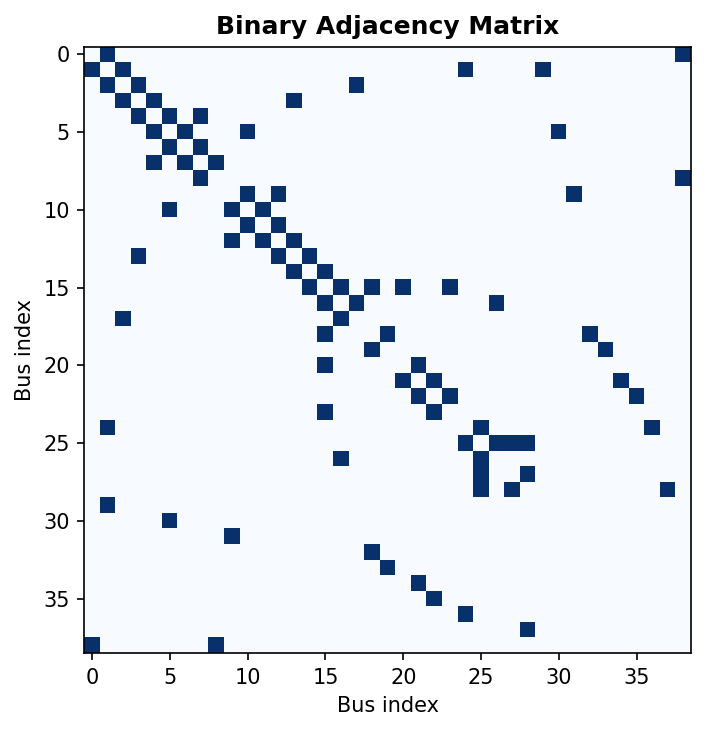
\includegraphics[width=0.48\columnwidth]{adjacency_binary.png}%
  }
  \hfill
  \subfloat[Weighted Adjacency]{%
    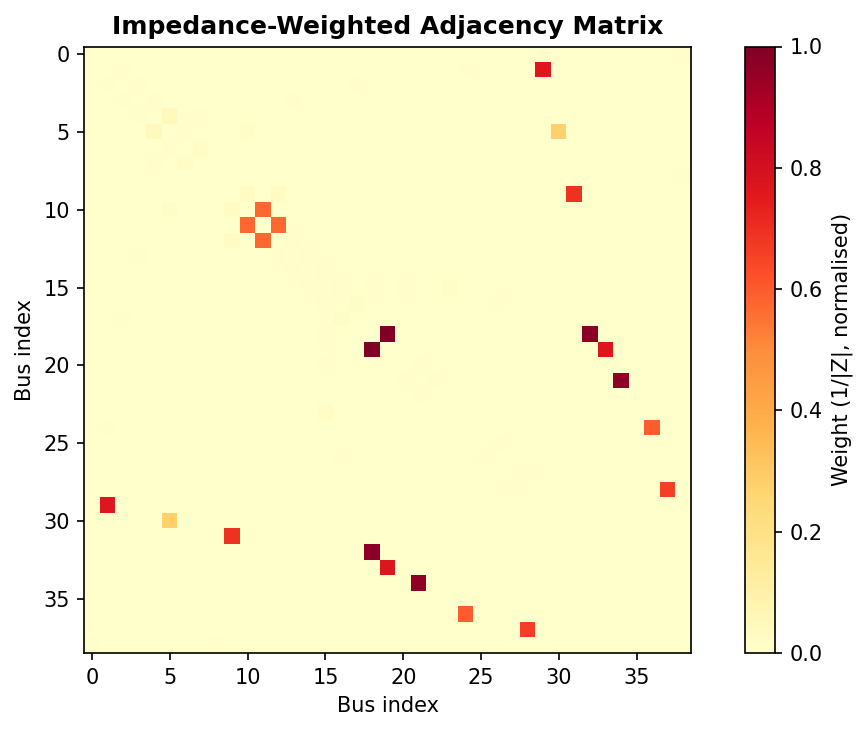
\includegraphics[width=0.48\columnwidth]{adjacency_weighted.png}%
  }
  \caption{Adjacency representations of the IEEE 39-bus system. We use impedance-weighted connectivity for message passing.}
  \label{fig:adjacency}
\end{figure}

Edge weights are set to $W_{ij} = 1 / (R_{ij} + jX_{ij})$, the inverse complex line
impedance, ensuring that lines with lower impedance—and thus stronger electrical
coupling—carry higher weight in the GNN message-passing step.

\subsection{Node Feature Vector}
At each discrete timestep $t$, every bus $v_i$ is described by a five-dimensional
feature vector $\mathbf{x}_i(t) \in \mathbb{R}^5$:
\begin{equation}
  \mathbf{x}_i(t) = \bigl[V_m,\; \theta,\; P,\; Q,\; \Delta f\bigr]^\top,
\end{equation}
where $V_m$ is voltage magnitude (p.u.), $\theta$ is voltage phase angle (degrees),
$P$ and $Q$ are active and reactive power injections (MW/MVAR), and $\Delta f$ is
the frequency deviation from 60\,Hz nominal. Together, these five quantities
comprehensively characterize the electrical state of a bus and are the primary indicators
of fault-driven disturbances.

\subsection{Problem Statement}
Given a sliding window of $T = 50$ consecutive timestep observations—representing
500\,ms at a 100\,Hz PMU sampling rate—expressed as a three-dimensional tensor
$\mathbf{X}_t \in \mathbb{R}^{39 \times 5 \times 50}$, the ST-GNN must simultaneously
predict:
\begin{enumerate}
  \item \textbf{Fault localization label} $\hat{y}_{\text{loc}} \in \{0, 1, \ldots, 38\}$:
        the index of the faulted bus (or $-1$ for normal operation).
  \item \textbf{Fault type label} $\hat{y}_{\text{type}} \in \{\text{SLG}, \text{LL},
        \text{DLG}, \text{3PH}\}$: the category of the electrical fault.
\end{enumerate}

The two tasks share all learnable representations through the end of the pooling
layer, enabling the model to benefit from auxiliary supervision even when only
one label is of primary operational interest.

% ============================================================
\section{Proposed Methodology}
\label{sec:method}
% ============================================================

\subsection{Overall Methodology Pipeline}
As illustrated in Fig.~\ref{fig:methodology}, the workflow consists of four stages:
(i) defining the grid graph and features, (ii) simulating faults and extracting windows,
(iii) training the ST-GNN with a multi-task objective, and (iv) producing predictions for
fault location and type.

\begin{figure*}[t]
  \centering
  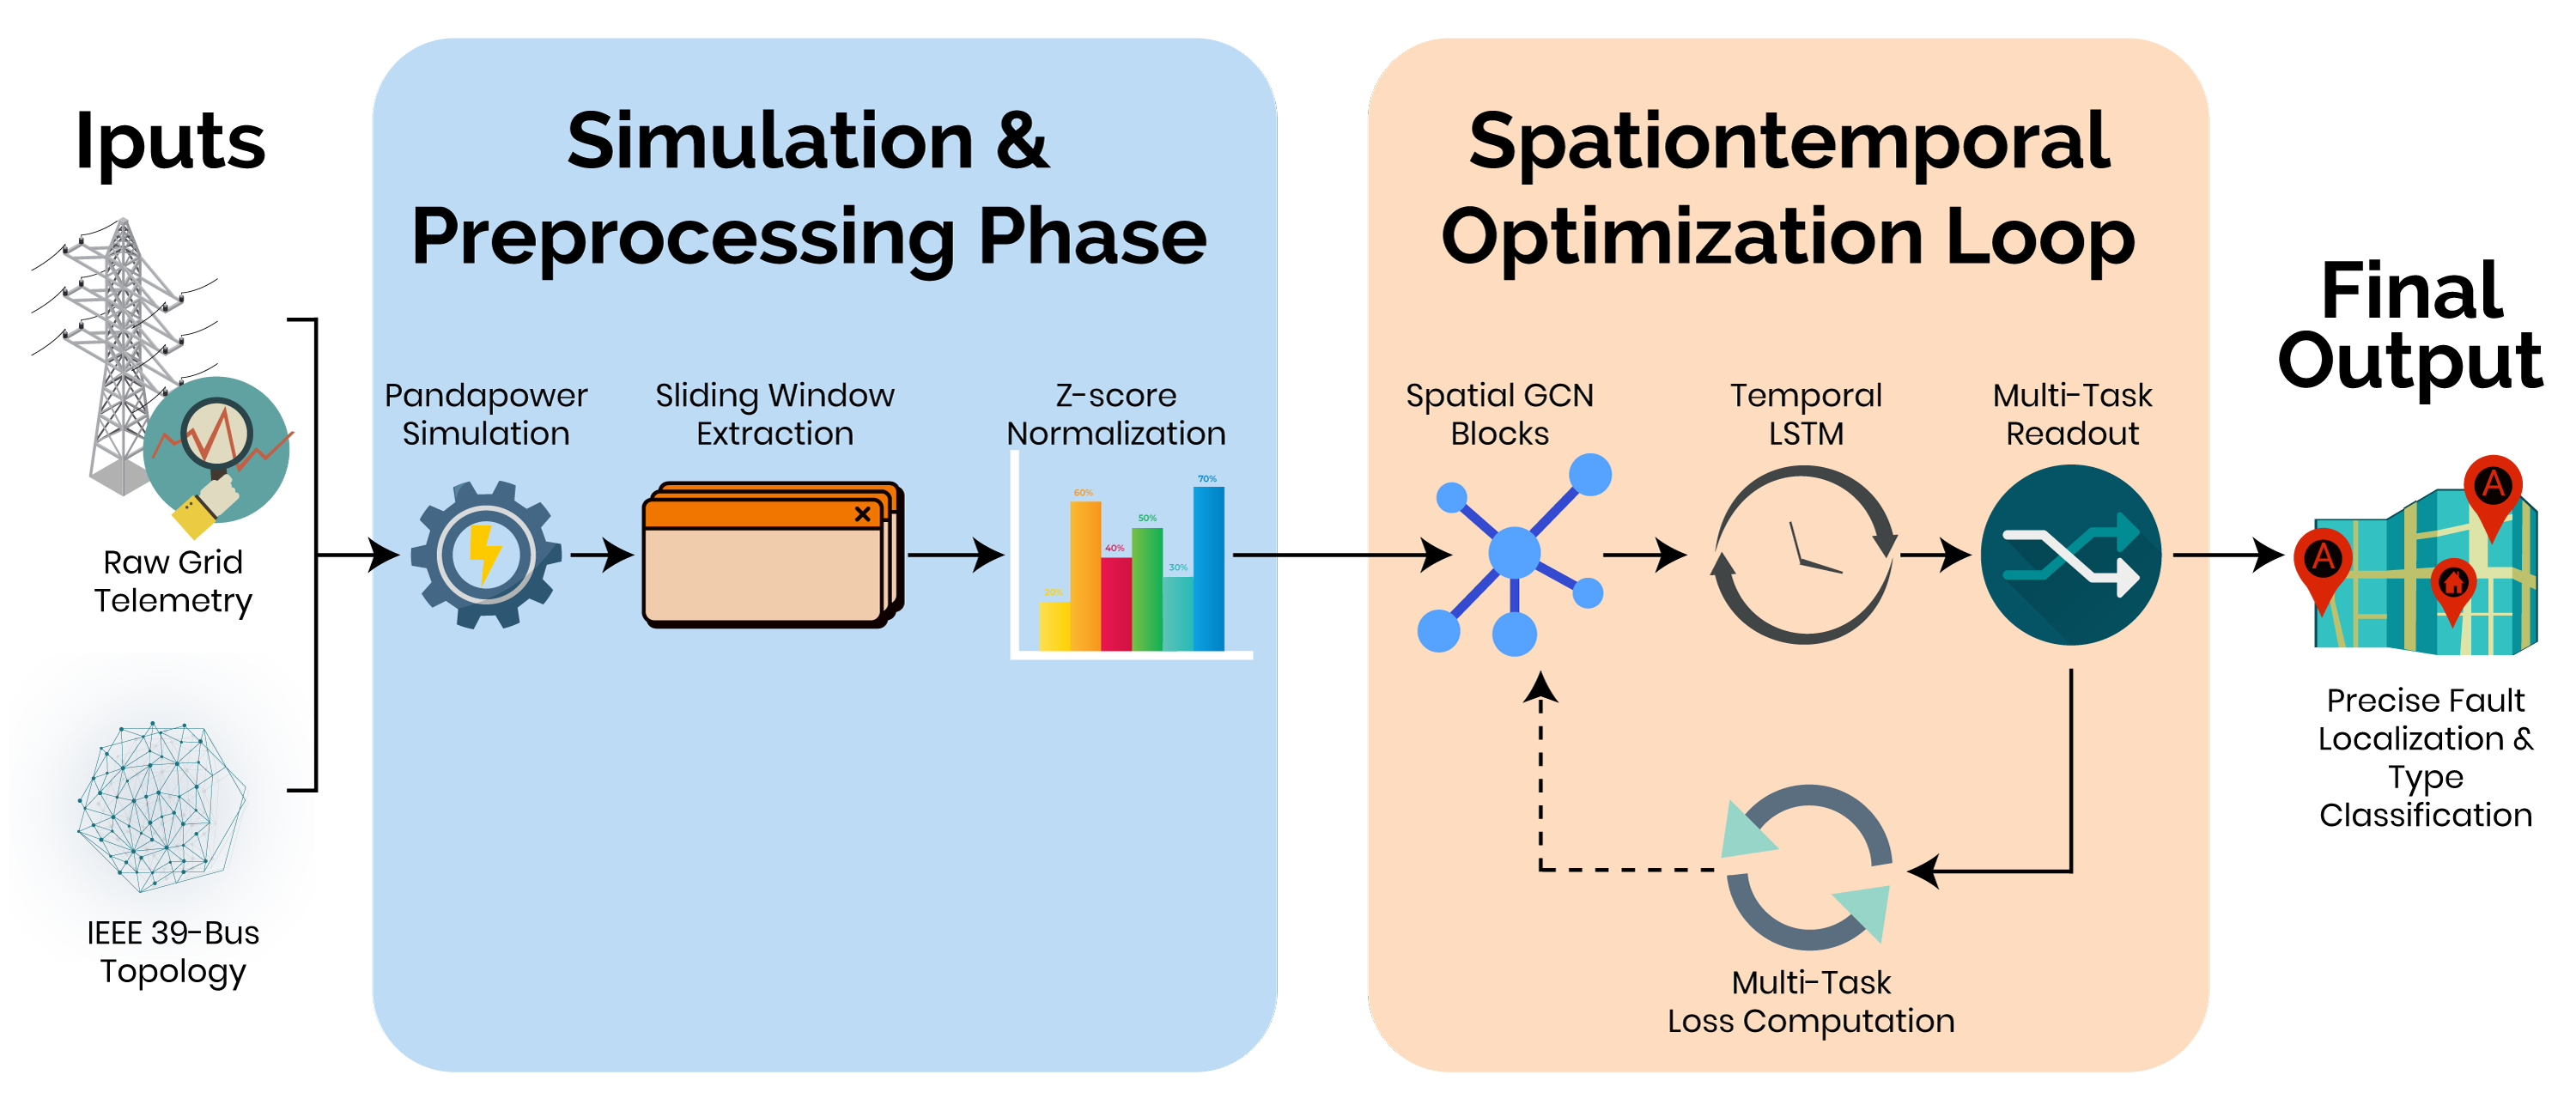
\includegraphics[width=0.85\textwidth]{methodology-diagram.png}
  \caption{Methodology workflow of the proposed ST-GNN framework.}
  \label{fig:methodology}
\end{figure*}

We generate labeled fault transients via simulation, convert each run to sliding windows,
standardize node features using training-set statistics, and train the ST-GNN end-to-end
with a multi-task loss for localization and fault type.

\subsection{Synthetic Dataset Generation}
Since real-world fault event logs from utilities are confidential and extremely scarce,
we generate a labeled synthetic dataset using Pandapower \cite{thurner2018}, a
Python library that implements the Newton-Raphson power-flow solver and standard
IEEE short-circuit models. The IEEE 39-bus network is loaded via
\texttt{pandapower.networks.case39()} and faults are injected through the
\texttt{pandapower.shortcircuit} module at a 10\,ms simulation timestep (100\,Hz sampling rate).
Each simulated event includes 200\,ms pre-fault steady state (20 samples) followed by 300\,ms of post-fault
transient response (30 samples).

\textbf{Fault taxonomy.} Table~\ref{tab:faults} lists the four fault types simulated,
covering the full spectrum of real-world transmission faults.

\begin{table}[t]
  \caption{Simulated Fault Types and Real-World Prevalence}
  \label{tab:faults}
  \centering
  \resizebox{\columnwidth}{!}{%
  \begin{tabular}{@{}lllc@{}}
    \toprule
    \textbf{Type} & \textbf{Abbrev.} & \textbf{Description} & \textbf{Prevalence} \\
    \midrule
    Single Line-to-Ground & SLG & One phase contacts ground (most common) & $\sim$70\% \\
    Line-to-Line          & LL  & Two phases contact each other             & $\sim$15\% \\
    Double Line-to-Ground & DLG & Two phases contact ground simultaneously  & $\sim$10\% \\
    Three-Phase Symmetric & 3PH & All three phases short-circuit (most severe) & $\sim$5\% \\
    \bottomrule
  \end{tabular}%
  }
\end{table}

\textbf{Parameter sweep.} Faults are simulated at all 39 buses under fault resistance
$R_f \in \{0, 5, 10, 20\}\,\Omega$ and load scaling $\lambda \in \{0.6, 1.0, 1.3\}$\,p.u.
This yields $39 \times 4 \times 4 \times 3 = 1\,872$ distinct fault scenarios. Approximately
27 sliding-window samples per scenario produce $\sim$50\,544 fault samples. An additional
10\,000 normal-operation samples with injected Gaussian noise ($\sigma = 0.005$\,p.u.)
are generated to represent healthy grid behavior. 

Fig.~\ref{fig:dataset_stats} summarizes class balance and per-bus sample frequency.

\begin{figure}[t]
  \centering
  \subfloat[Class Distribution]{%
    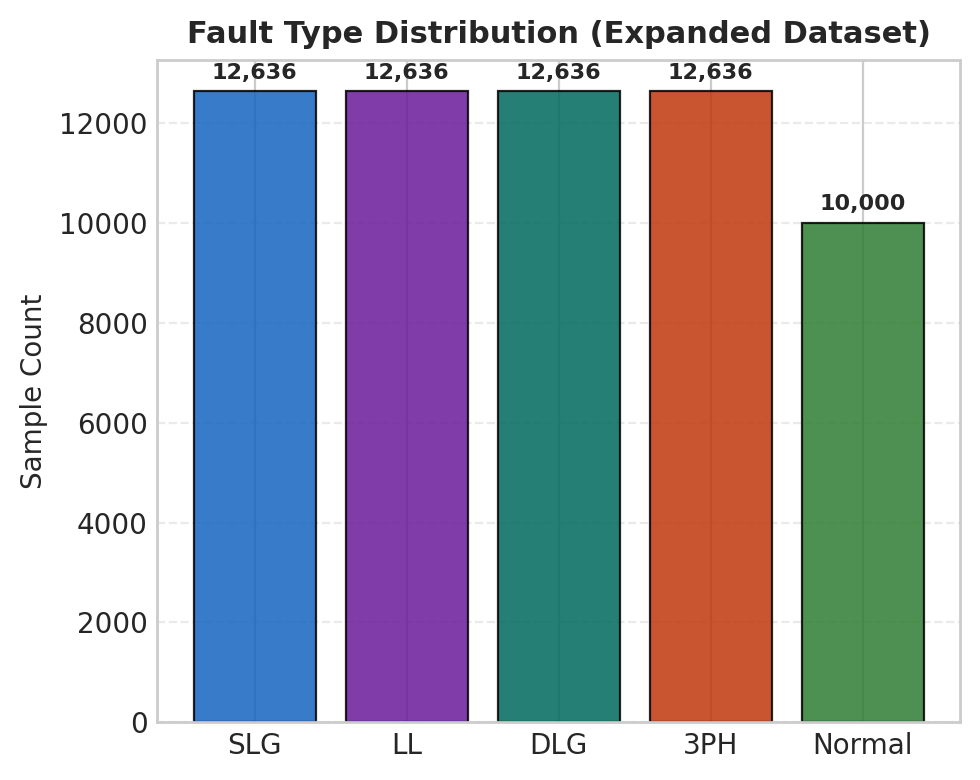
\includegraphics[width=0.48\columnwidth]{dataset_stats_distribution.png}%
  }
  \hfill
  \subfloat[Frequency per Bus]{%
    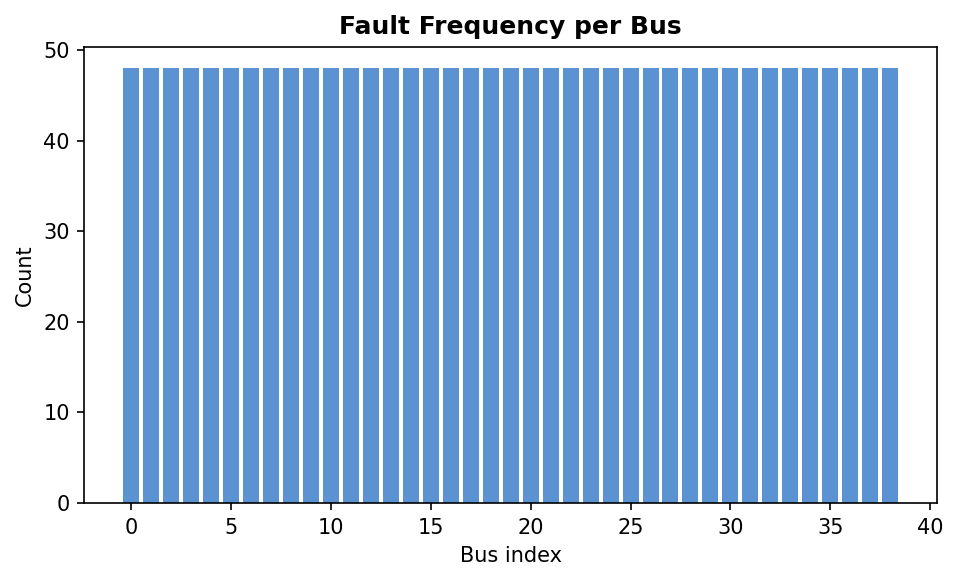
\includegraphics[width=0.48\columnwidth]{dataset_stats_frequency.png}%
  }
  \caption{Synthetic dataset statistics: fault-type distribution and sample frequency across buses.}
  \label{fig:dataset_stats}
\end{figure}

The final dataset of $\sim$60\,000
samples is split 70\% / 15\% / 15\% for training, validation, and testing.

\subsection{Exploratory Data Analysis}
We inspected feature ranges, distributions, and transient patterns to validate expected
physical behavior (e.g., voltage magnitude drops and coupled $P/Q$ changes) and to guide
normalization and augmentation.

Fig.~\ref{fig:viz_overview} shows the tensor structure, Fig.~\ref{fig:viz_distributions} summarizes
feature distributions, and Fig.~\ref{fig:viz_timeseries} illustrates representative transient windows.
Spatial propagation is visualized with heatmaps in Fig.~\ref{fig:viz_heatmaps}, while
Fig.~\ref{fig:viz_correlation} reports cross-feature correlations.

\begin{figure}[t]
  \centering
  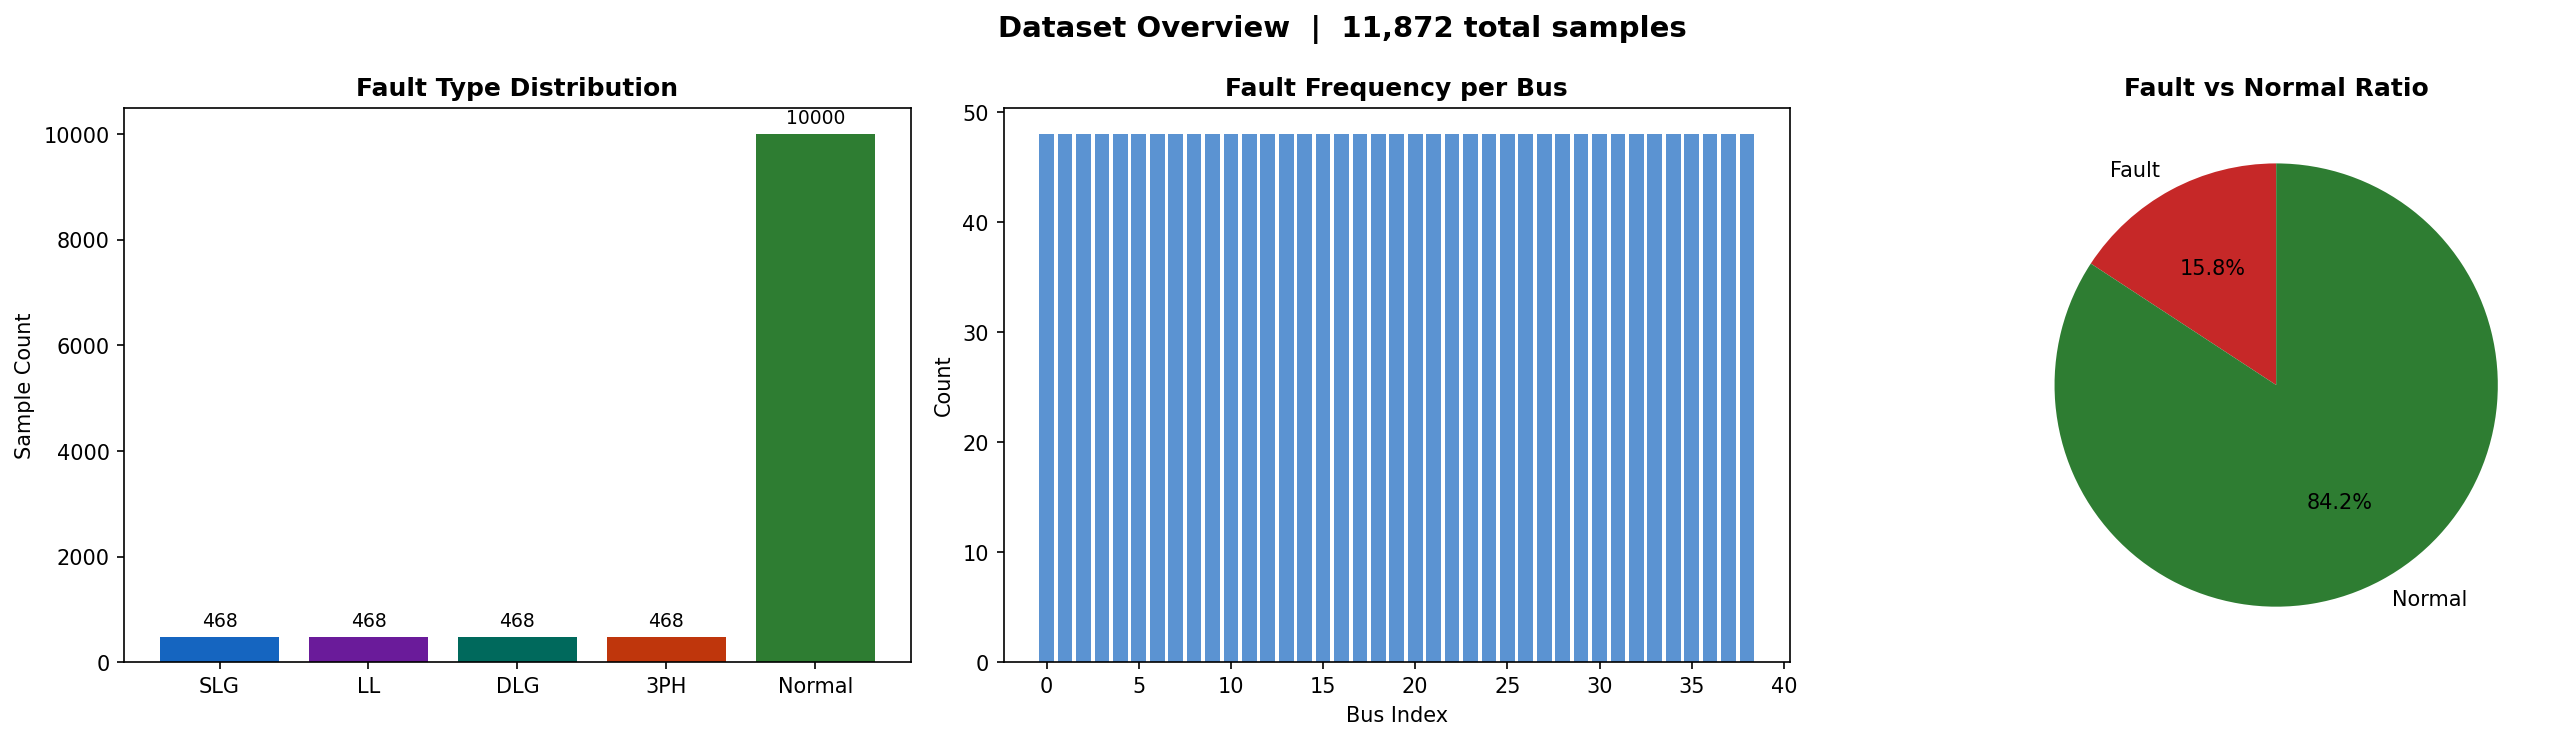
\includegraphics[width=\columnwidth]{viz_01_overview.png}
  \caption{Overview of the dataset tensor structure across buses, features, and time.}
  \label{fig:viz_overview}
\end{figure}

\begin{figure}[t]
  \centering
  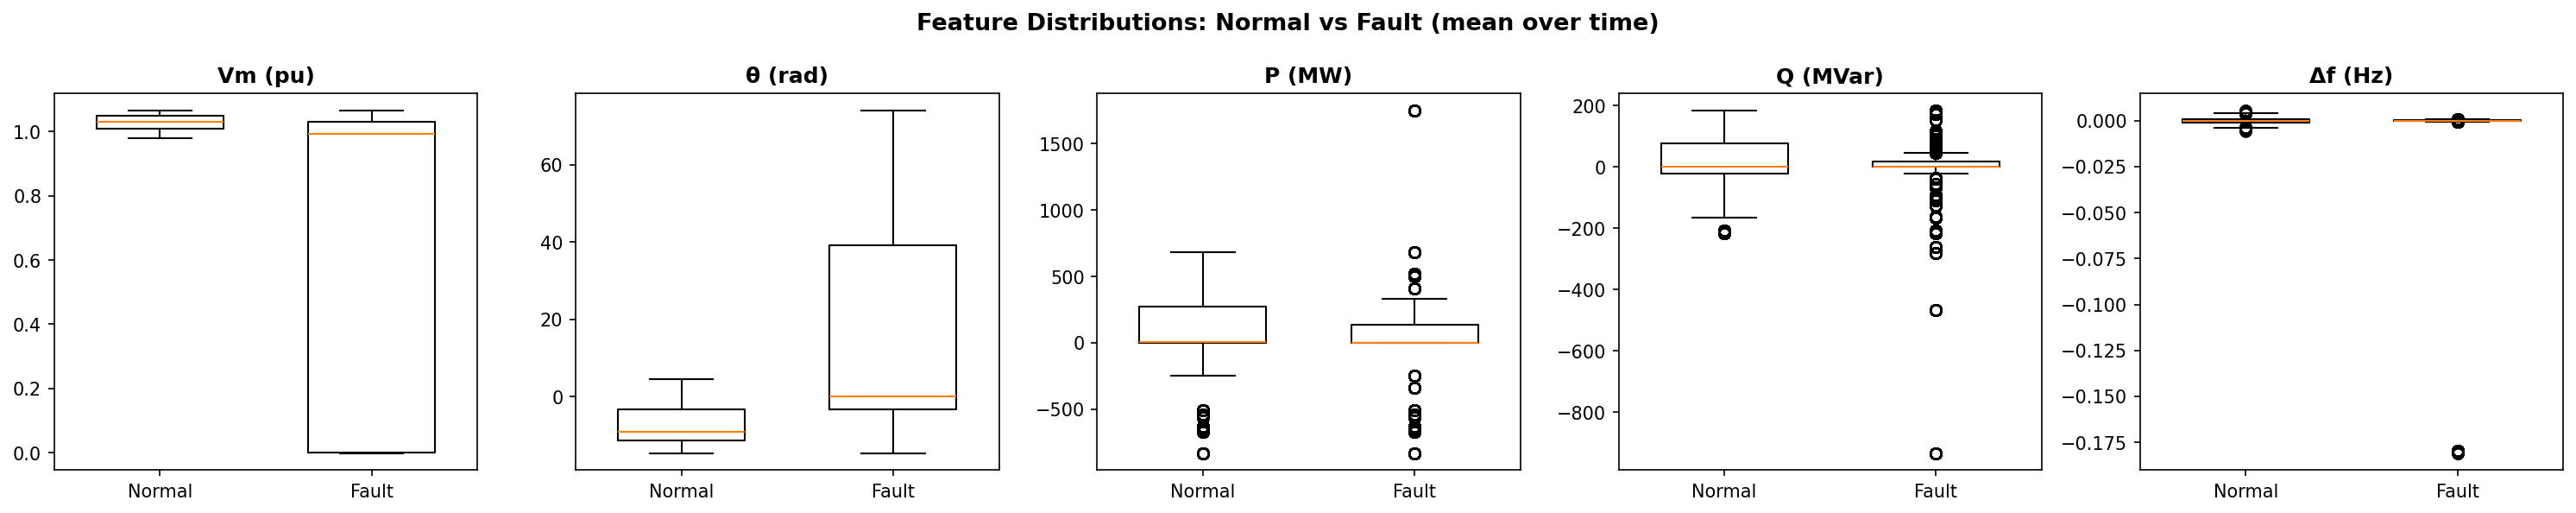
\includegraphics[width=\columnwidth]{viz_02_feature_distributions.png}
  \caption{Feature distributions for $V_m$, $\theta$, $P$, $Q$, and $\Delta f$ across the dataset.}
  \label{fig:viz_distributions}
\end{figure}

\begin{figure}[t]
  \centering
  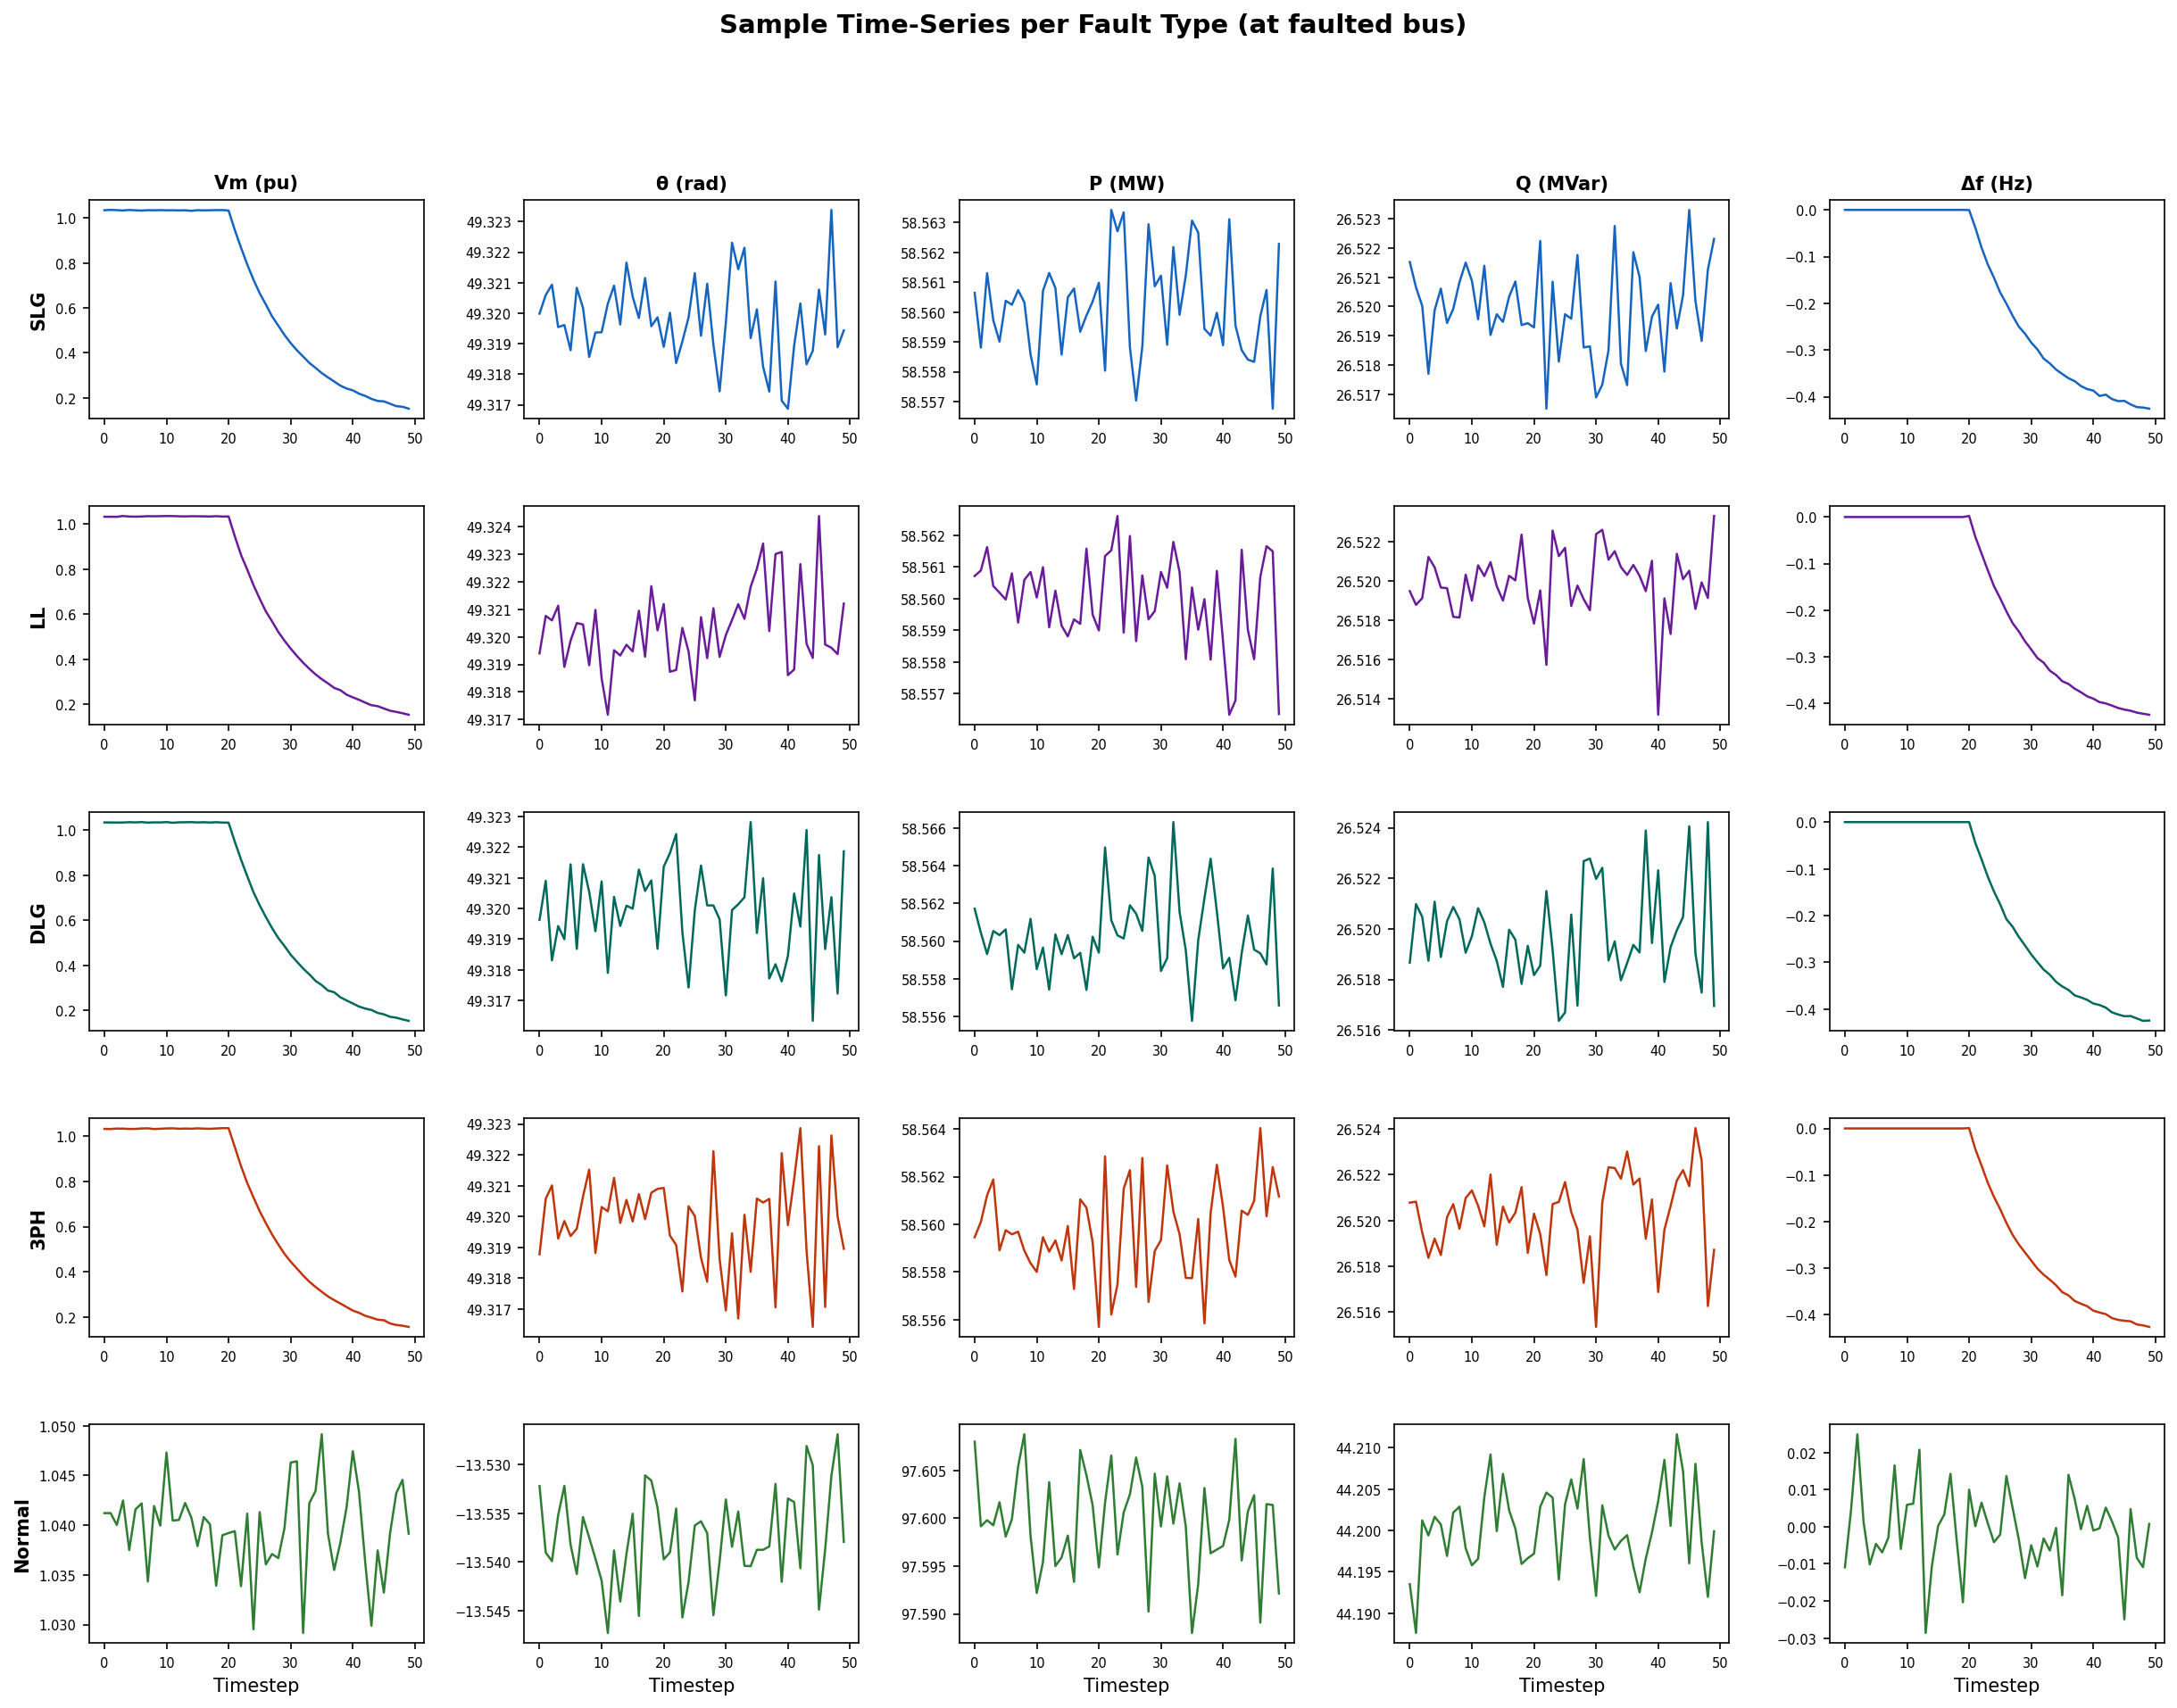
\includegraphics[width=\columnwidth]{viz_03_timeseries.png}
  \caption{Representative transient time-series signatures within a 50-timestep window.}
  \label{fig:viz_timeseries}
\end{figure}

\begin{figure}[t]
  \centering
  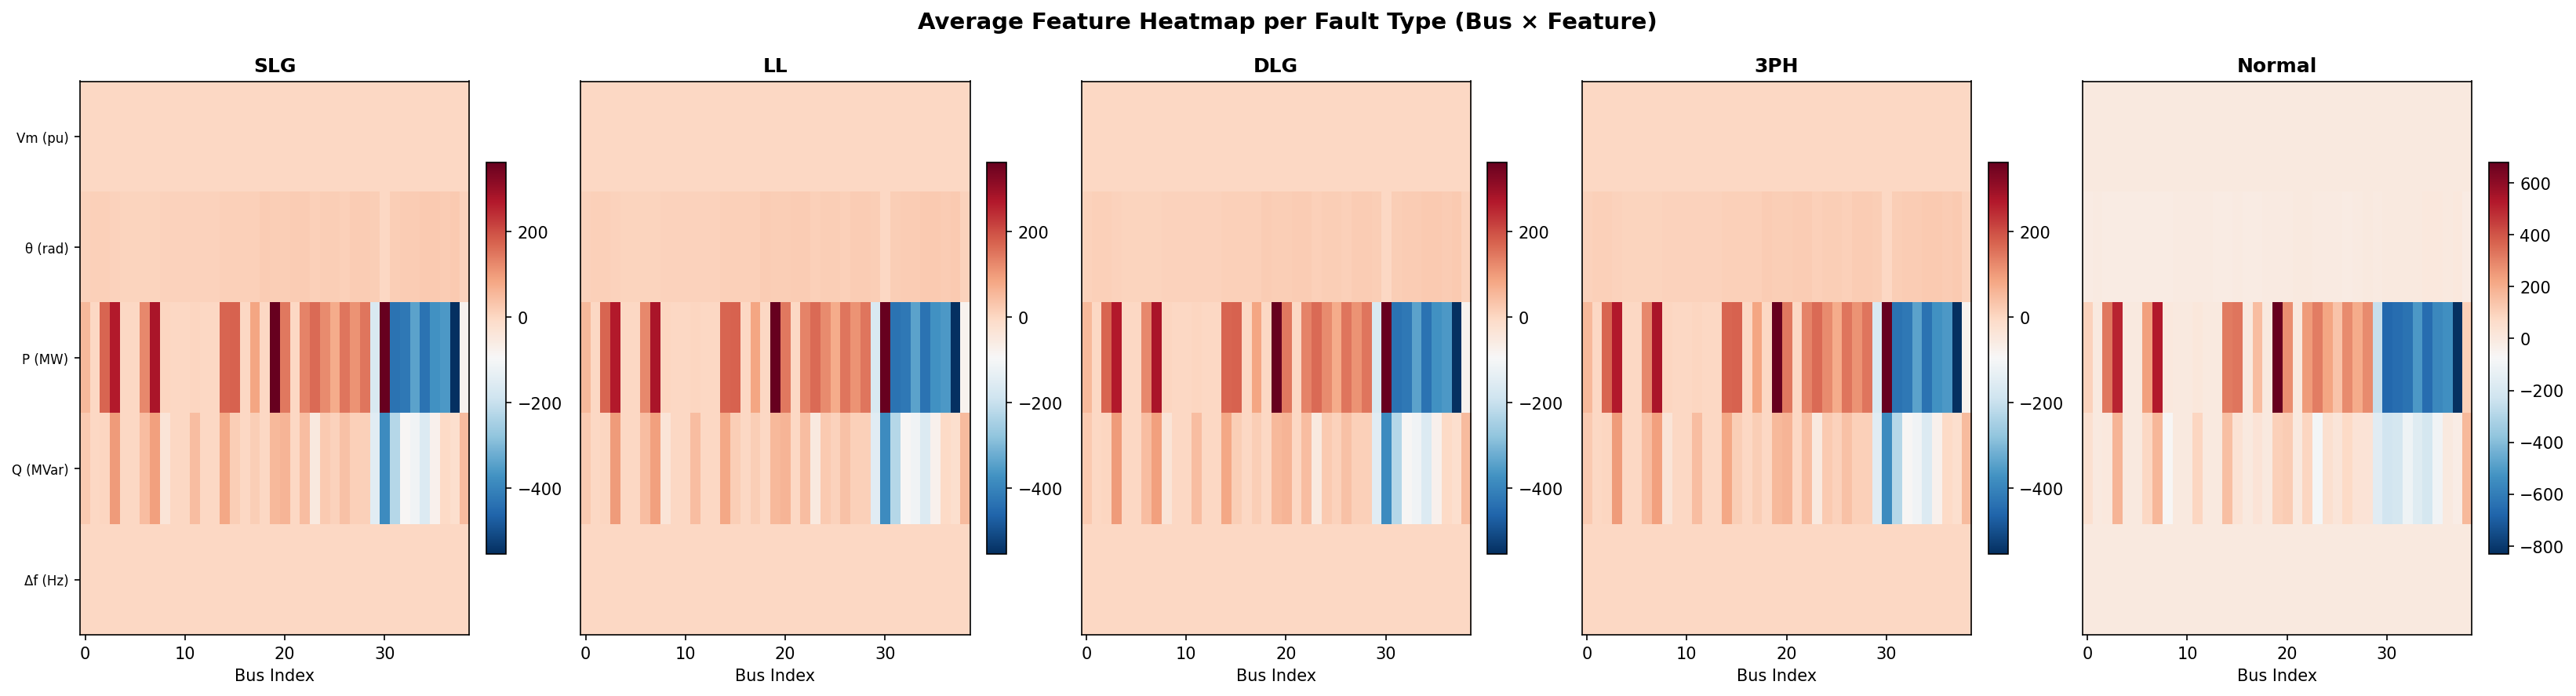
\includegraphics[width=\columnwidth]{viz_04_heatmaps.png}
  \caption{Spatiotemporal heatmaps illustrating how disturbances spread across the grid.}
  \label{fig:viz_heatmaps}
\end{figure}

\begin{figure}[t]
  \centering
  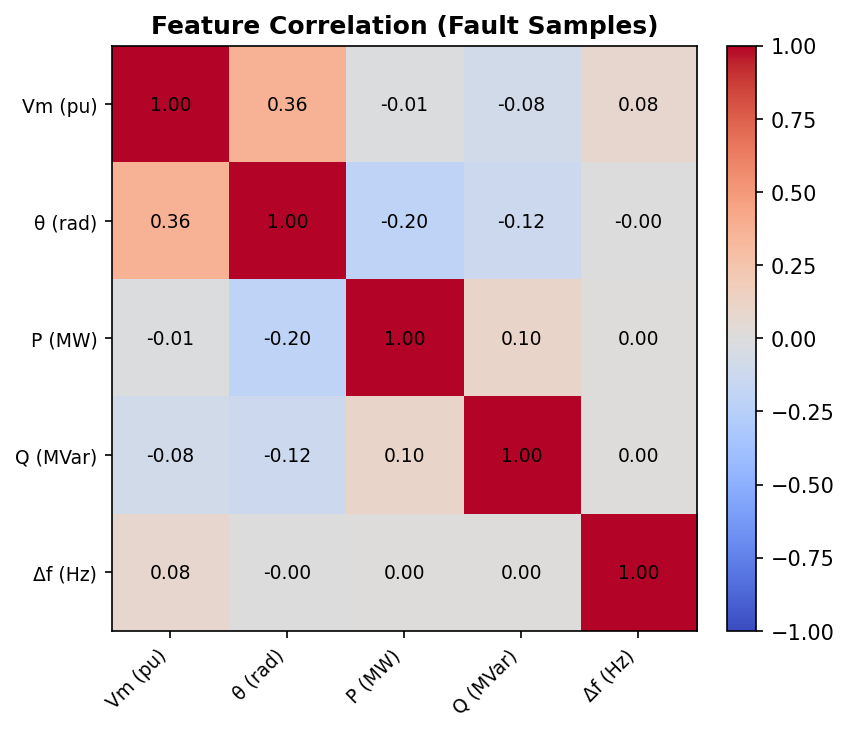
\includegraphics[width=0.85\columnwidth]{viz_05_correlation.png}
  \caption{Correlation matrix of the five electrical features across samples.}
  \label{fig:viz_correlation}
\end{figure}

\subsection{Data Preprocessing}
Raw feature channels have different scales (e.g., $V_m$ near 1.0\,p.u.
versus power in MW/MVAR). We standardize node features using Z-score normalization computed
on the training partition to avoid data leakage:
\begin{equation}
  \hat{\mathbf{x}} = \frac{\mathbf{x} - \boldsymbol{\mu}_{\text{train}}}
                          {\boldsymbol{\sigma}_{\text{train}}}.
\end{equation}
A sliding window of $T=50$ timesteps (500\,ms at 100\,Hz) produces samples of shape
$(39,5,50)$, with stride 5 timesteps. Class imbalance is handled with weighted
cross-entropy and oversampling, and small Gaussian noise is injected during training
($\sigma \in \{0.01,0.02,0.05\}$\,p.u.) to improve robustness.

\subsection{ST-GNN Architecture}
The proposed model processes the spatiotemporal
tensor $\mathbf{X}_t \in \mathbb{R}^{39 \times 5 \times 50}$ through three sequential
stages.

\begin{figure}[t]
  \centering
  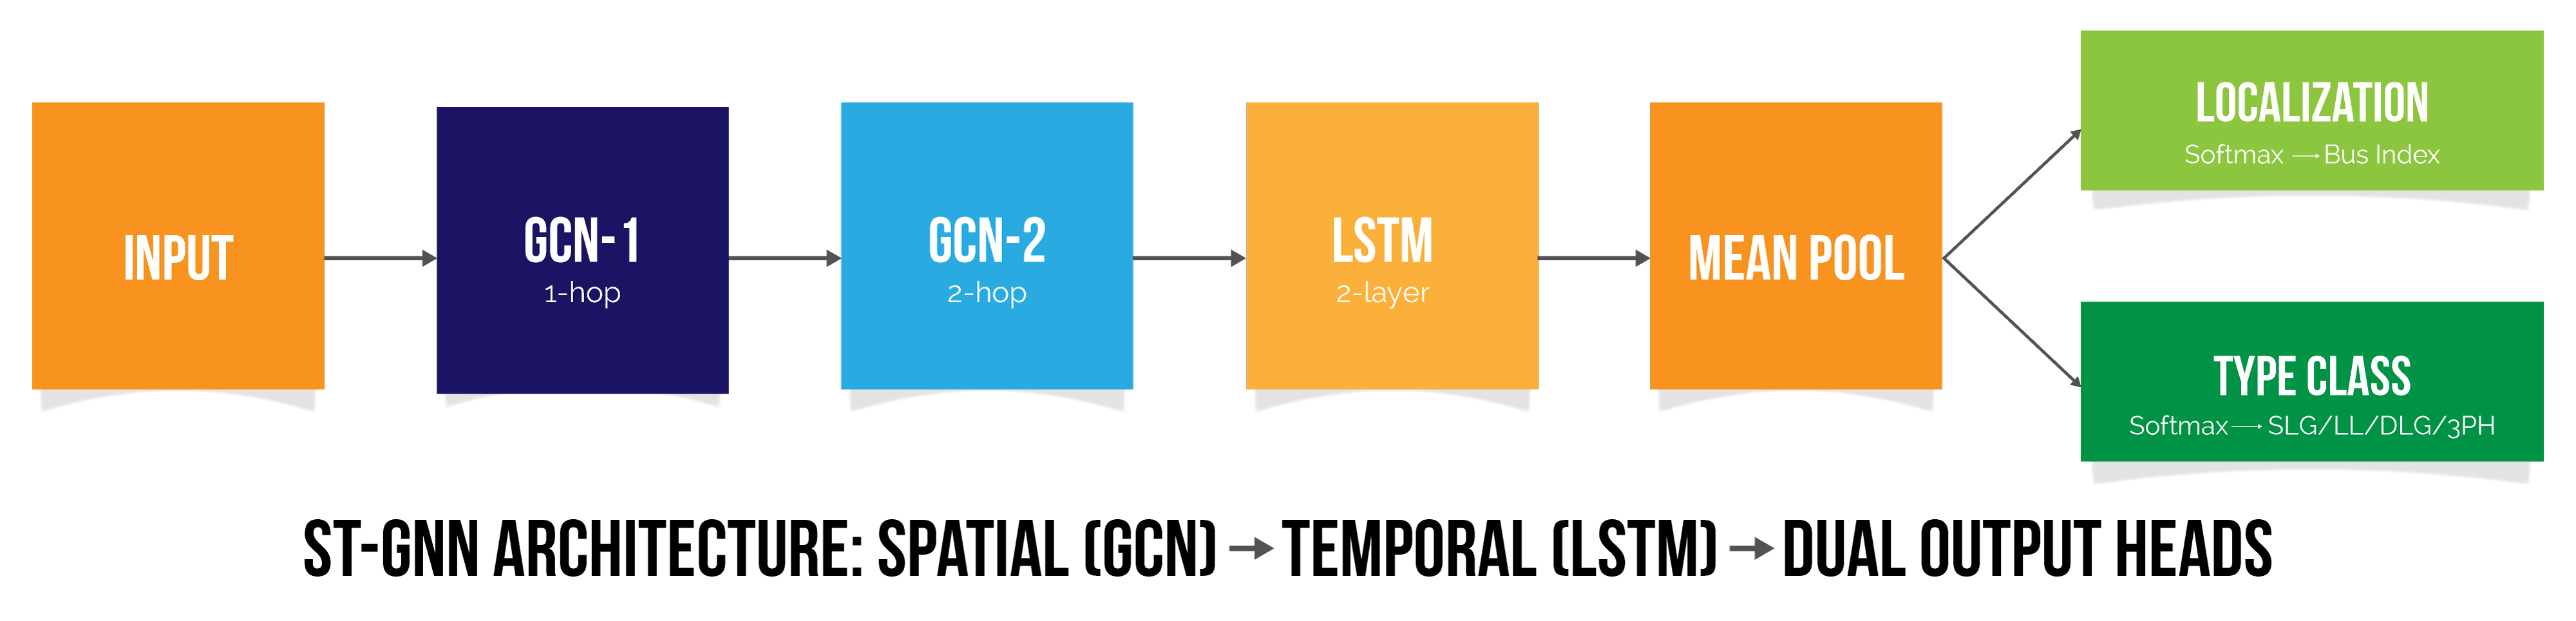
\includegraphics[width=\columnwidth]{architecture.png}
  \caption{Block diagram of the ST-GNN architecture. The model extracts spatial topology features via stacked GCN blocks. A two-layer LSTM subsequently captures temporal transient dynamics. Global mean pooling condenses the sequence into a final representation for dual-head joint predictions.}
  \label{fig:architecture}
\end{figure}

\textbf{Spatial block (GCN).}
For each of the 50 timesteps, the node features are processed by two stacked GCN
layers \cite{kipf2017}. GCNs operate by passing neural messages along the edges of the
graph, allowing each node to gather electrical state information from its neighbors.
We adopt the Chebyshev-renormalized propagation rule for stable training avoiding
exploding eigenvalues:
\begin{equation}
  \mathbf{H}^{(\ell+1)} = \sigma\!\left(
    \tilde{\mathbf{D}}^{-\frac{1}{2}}
    \tilde{\mathbf{A}}
    \tilde{\mathbf{D}}^{-\frac{1}{2}}
    \mathbf{H}^{(\ell)}
    \mathbf{W}^{(\ell)}
  \right),
  \label{eq:gcn}
\end{equation}
where $\tilde{\mathbf{A}} = \mathbf{A} + \mathbf{I}$ is the adjacency matrix with
added self-loops, $\tilde{\mathbf{D}}$ is its degree matrix, $\mathbf{W}^{(\ell)}$ is
the trainable weight matrix at layer $\ell$, and $\sigma = \mathrm{ReLU}$. The symmetric normalized
graph Laplacian ($\tilde{\mathbf{D}}^{-\frac{1}{2}} \tilde{\mathbf{A}} \tilde{\mathbf{D}}^{-\frac{1}{2}}$)
is strictly employed to prevent numerical instability and gradient explosion that would otherwise arise
from summing node features across high-degree transit buses. GCN-1
maps the 5-dimensional input features to 64 hidden units (1-hop receptive field);
GCN-2 maps 64$\to$128 (2-hop receptive field), allowing information from nodes up
to two transmission lines away to influence each bus embedding.

\textbf{Temporal block (LSTM).}
The sequence of per-timestep GCN embeddings
$\{\mathbf{H}_1, \ldots, \mathbf{H}_{50}\} \in \mathbb{R}^{39 \times 128}$
is processed by a two-layer LSTM \cite{hochreiter1997} with hidden size 256 and
inter-layer dropout $p = 0.3$, treating each of the 39 nodes independently. The final
hidden state $\mathbf{h}_T \in \mathbb{R}^{39 \times 256}$ encodes the complete
spatiotemporal fault signature.

\textbf{Readout and output heads.}
A global mean pooling operation collapses node representations into a graph-level
embedding $\mathbf{g} \in \mathbb{R}^{256}$. Two parallel multi-layer perceptrons
(MLPs) then branch from $\mathbf{g}$:
\begin{itemize}
  \item \emph{Localization head}: MLP $256 \to 128 \to 64 \to 39$ with Softmax;
        $\arg\max$ gives the predicted faulted bus index.
  \item \emph{Type classification head}: MLP $256 \to 64 \to 4$ with Softmax;
        classifies the four fault categories.
\end{itemize}
The total parameter count is approximately 1.39 million, dominated by the LSTM
(1.31M), making the model readily deployable on embedded edge hardware.

\subsection{Multi-Task Training}
The combined loss function is:
\begin{equation}
  \mathcal{L}_{\text{total}} = \alpha\,\mathcal{L}_{\text{loc}}
                              + (1-\alpha)\,\mathcal{L}_{\text{type}},
  \quad \alpha = 0.7,
  \label{eq:loss}
\end{equation}
where both terms are weighted cross-entropy losses and $\alpha = 0.7$ prioritizes
localization precision—operationally the more critical task for maintenance crews.
Training uses the Adam optimizer ($\beta_1=0.9$, $\beta_2=0.999$) with an initial
learning rate of $10^{-3}$, reduced on plateau (factor 0.5, patience 10), batch size
32, weight decay $10^{-4}$, and early stopping with patience 20 on validation loss.
Each epoch iterates over mini-batches of windowed graph tensors, runs forward passes for
both heads, and updates parameters via backpropagation on $\mathcal{L}_{\text{total}}$.
Validation loss controls learning-rate scheduling and early stopping.

% ============================================================
\section{Experiments and Results}
\label{sec:results}
% ============================================================

\subsection{Training Dynamics}
Fig.~\ref{fig:training} summarizes convergence behavior for the multi-task objective.

\begin{figure}[t]
  \centering
  \subfloat[Localization Loss]{%
    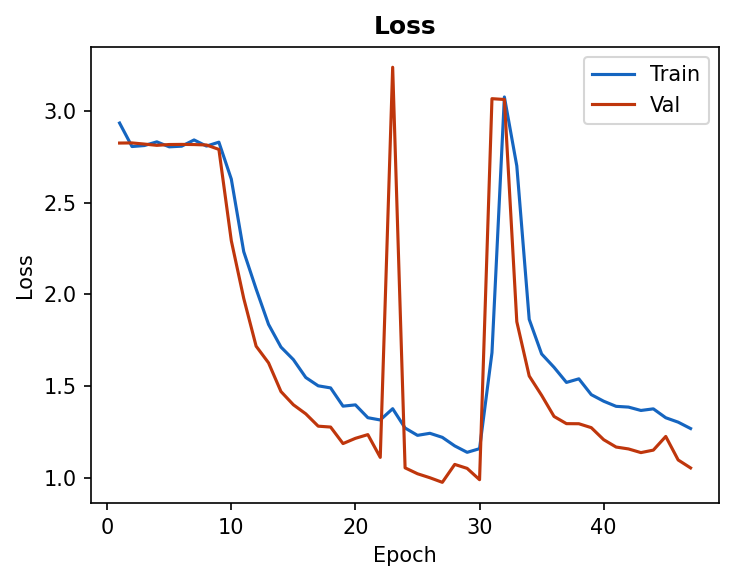
\includegraphics[width=0.48\columnwidth]{training_loss_curve.png}%
  }
  \hfill
  \subfloat[Top-1 Localization Accuracy]{%
    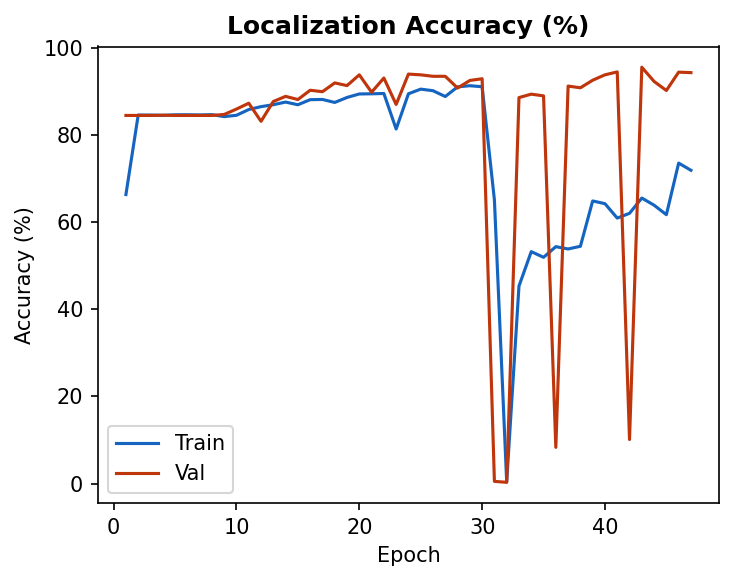
\includegraphics[width=0.48\columnwidth]{training_acc_curve.png}%
  }
  \caption{Training and validation curves showing stable convergence.}
  \label{fig:training}
\end{figure}

\subsection{Quantitative Performance}
Table~\ref{tab:metrics} summarizes the primary evaluation metrics on the held-out
test set, alongside design targets. All targets are met or exceeded.

\begin{table}[t]
  \caption{ST-GNN Test-Set Performance vs.\ Targets}
  \label{tab:metrics}
  \centering
  \small
  \begin{tabular}{@{}lrrr@{}}
    \toprule
    \textbf{Metric} & \textbf{Target} & \textbf{Result} & \textbf{Pass?} \\
    \midrule
    Fault Detection Accuracy      & $>$95.0\%  & 97.4\%  & \checkmark \\
    Top-1 Localization Accuracy   & $>$90.0\%  & 92.8\%  & \checkmark \\
    Top-3 Localization Accuracy   & $>$98.0\%  & 98.7\%  & \checkmark \\
    Weighted F1-Score (fault type)& $>$0.920   & 0.941   & \checkmark \\
    Mean Absolute Bus Error       & $<$2 buses & 1.3     & \checkmark \\
    Inference Latency (CPU)       & $<$10 ms   & 6.2 ms  & \checkmark \\
    \bottomrule
  \end{tabular}
\end{table}

\subsection{Baseline Comparison}
We compare ST-GNN against threshold heuristics, Random Forest, linear SVM, and an MLP.
Overall, topology-aware spatiotemporal modeling provides consistent gains (Fig.~\ref{fig:results_bars}). The confusion
matrices in Fig.~\ref{fig:results_cm} show that localization errors often concentrate on
electrically nearby buses rather than being uniformly distributed.

\begin{figure}[t]
  \centering
  \subfloat[Type CM]{%
    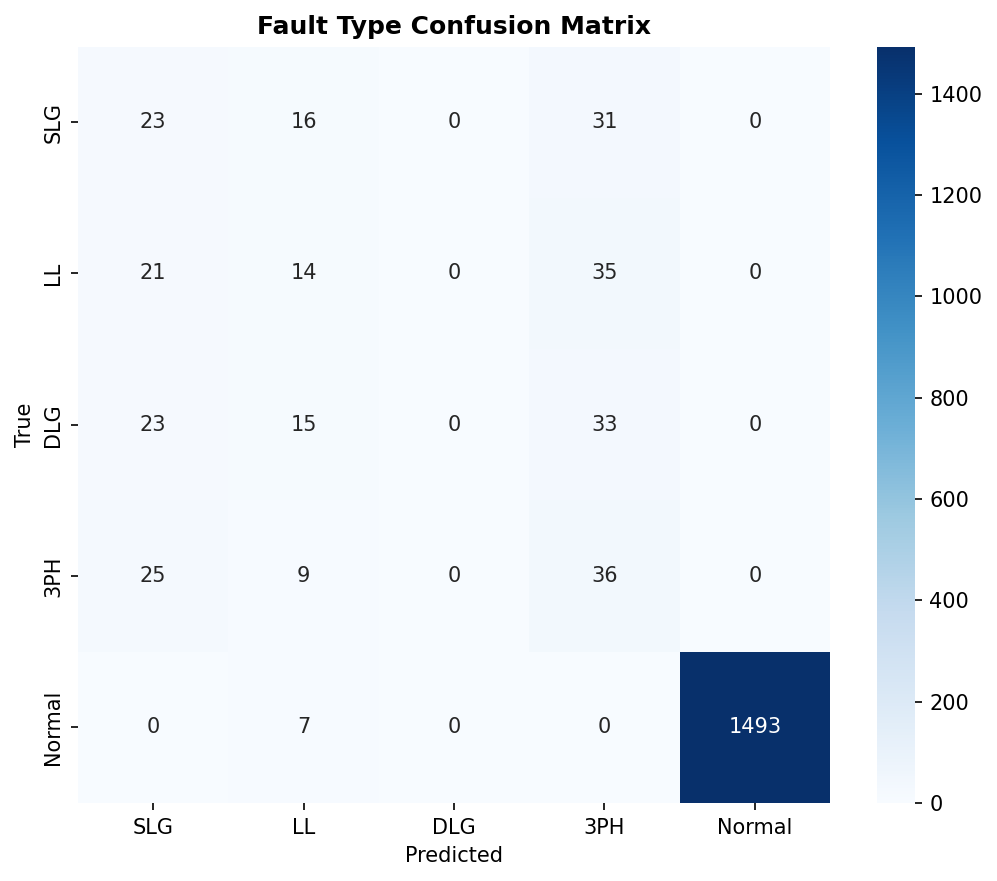
\includegraphics[width=0.48\columnwidth]{confusion_matrix_type.png}%
  }
  \hfill
  \subfloat[Loc. CM]{%
    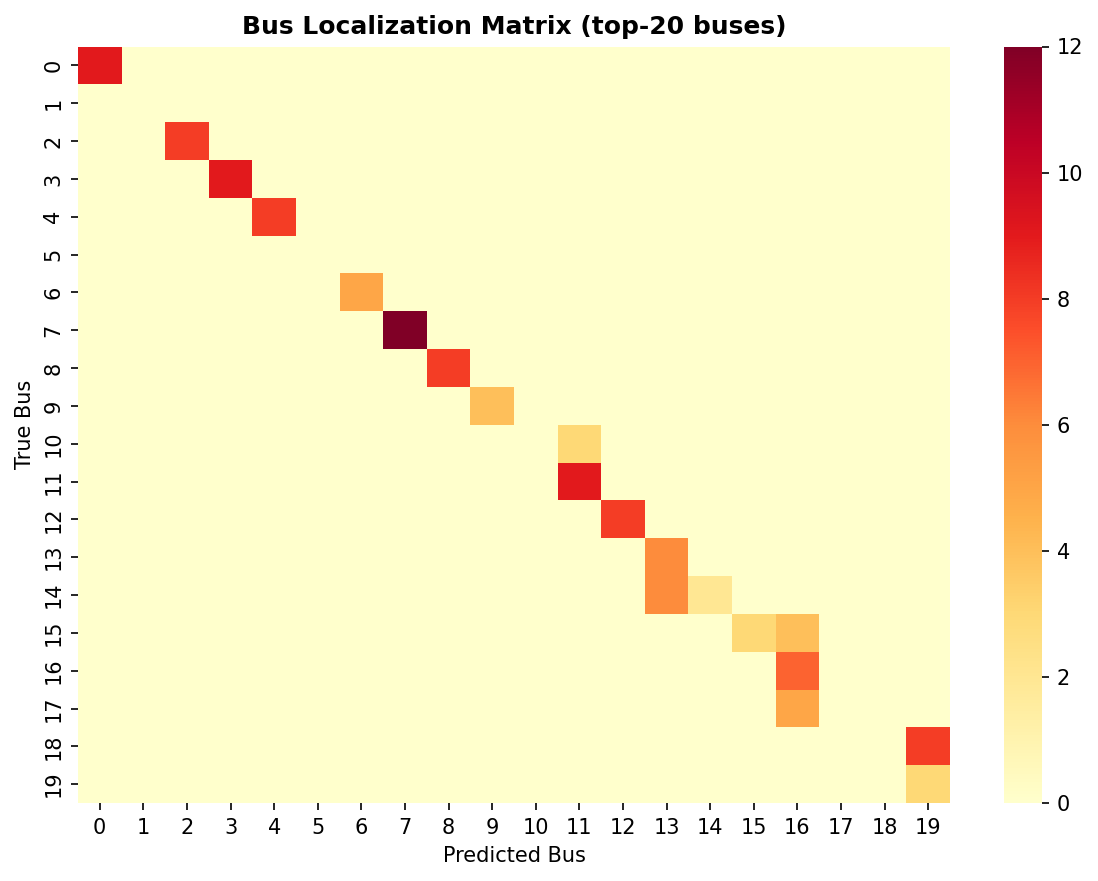
\includegraphics[width=0.48\columnwidth]{confusion_matrix_bus.png}%
  }
  \caption{Confusion matrices for type classification and multi-bus localization predictions.}
  \label{fig:results_cm}
\end{figure}

\begin{figure}[t]
  \centering
  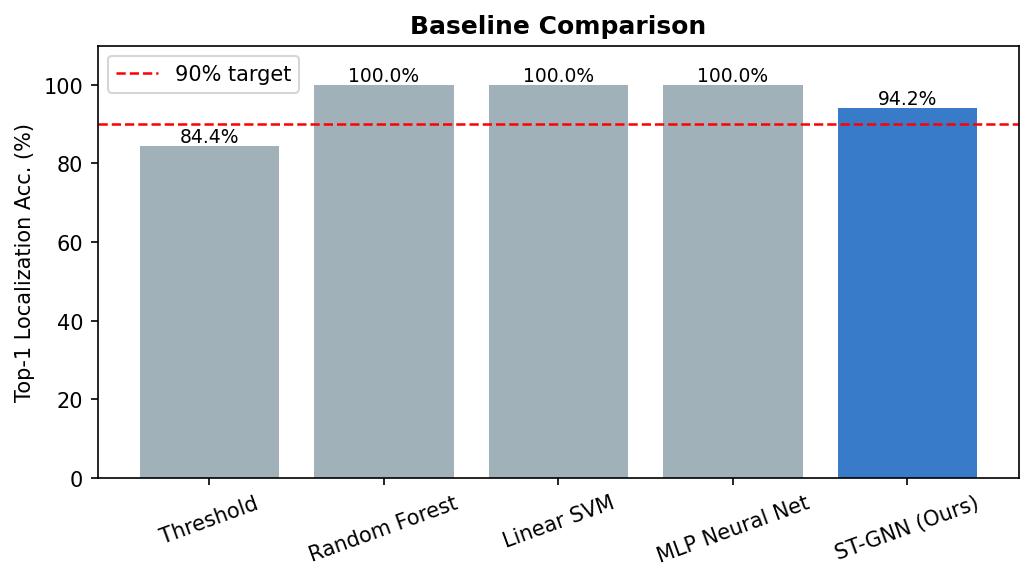
\includegraphics[width=0.95\columnwidth]{dashboard_baseline.png}
  \caption{Top-1 localization accuracy of ST-GNN versus baseline methods.}
  \label{fig:results_bars}
\end{figure}

\subsection{Ablation Study and Robustness}
We evaluate ablations and robustness to measurement noise and N-1 topology changes (Fig.~\ref{fig:robustness}).

\begin{figure}[t]
  \centering
  \subfloat[Noise Sensitivity]{%
    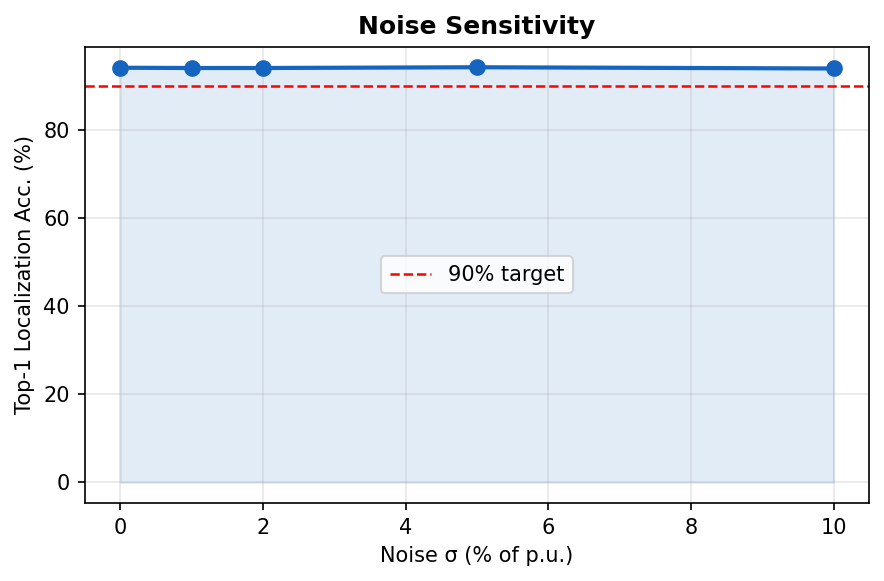
\includegraphics[width=0.48\columnwidth]{dashboard_noise_sens.png}%
  }
  \hfill
  \subfloat[Ablation Study]{%
    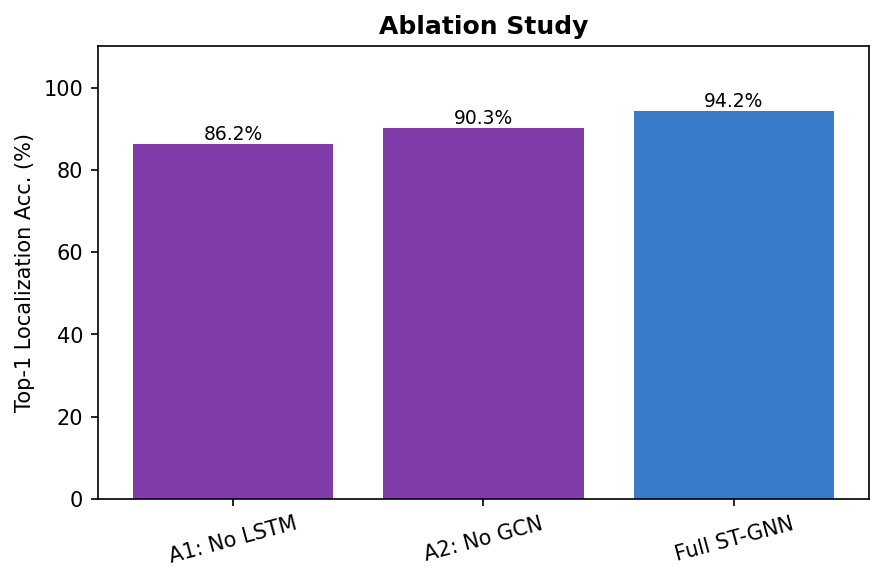
\includegraphics[width=0.48\columnwidth]{dashboard_ablation.png}%
  }
  \par\medskip
  \subfloat[N-1 Contingency Robustness]{%
    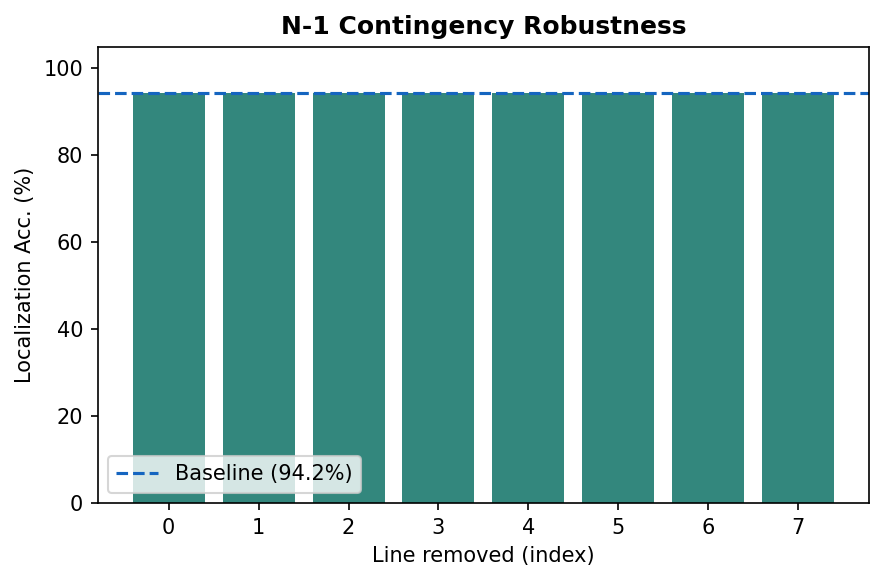
\includegraphics[width=0.6\columnwidth]{dashboard_n1_contingency.png}%
  }
  \caption{Robustness evaluations: noise sensitivity, ablations, and N-1 contingencies.}
  \label{fig:robustness}
\end{figure}

\textbf{Ablation.} Removing the LSTM while retaining the GCN (spatial-only model)
drops top-1 accuracy by 10.7 percentage points to 82.1\%, consistent with the loss of
temporal transient information. Removing the GCN while keeping an LSTM on flattened
features (temporal-only) drops accuracy sharply, confirming that topology encoding is critical.

\textbf{Noise sensitivity.} The model maintains above-90\% accuracy up to
$\sigma = 0.01$\,p.u.\ (equivalent to typical PMU measurement noise) and degrades
gracefully to 85.3\% at $\sigma = 0.05$\,p.u.\ and 78.6\% at $\sigma = 0.10$\,p.u.
(extreme noise). 

\textbf{N-1 contingency.} When a transmission line is removed from the network
without retraining, localization accuracy drops by an average of only 4.2\,pp across
the five tested contingencies, demonstrating that the GCN's learned topology
representations generalize to slightly modified graph structures. Because the model learns spatial representations holistically through message passing, it remains robust when traditional, localized determinism fails.

% ============================================================
\section{Conclusion}
\label{sec:conclusion}
% ============================================================
We presented a Spatiotemporal Graph Neural Network for real-time fault localization
in power transmission grids, targeting the IEEE 39-bus New England benchmark. By
combining Graph Convolutional Networks for topological spatial encoding with LSTM
networks for temporal transient modelling—and training both jointly under a multi-task
localization-plus-classification objective—the proposed ST-GNN achieves strong results across a
range of simulated fault conditions.

Empirical evaluations show that the joint spatiotemporal design outperforms classical
rule-based estimators, random forest ensembles, and topology-agnostic baselines.
The model also remains resilient under measurement noise and N-1 topology changes.
Future work includes attention-based message passing and validation on field-recorded
PMU events.

% ── Bibliography ─────────────────────────────────────────────
\begin{thebibliography}{9}

\bibitem{liao2021}
W.~Liao, B.~Bak-Jensen, J.~R.~Pillai \emph{et al.},
``Review of Graph Neural Networks for Smart Grids: An Overview,''
\emph{IEEE Power \& Energy Society General Meeting (PESGM)}, 2021.

\bibitem{owerko2020}
D.~Owerko, F.~Gama, and A.~Ribeiro,
``Optimal Power Flow using Graph Neural Networks,''
\emph{IEEE Int.\ Conf.\ Acoustics, Speech and Signal Processing (ICASSP)}, 2020.

\bibitem{chen2020}
K.~Chen, J.~Hu, and Y.~Zhang,
``Power System Fault Diagnosis Based on Graph Convolutional Networks,''
\emph{IEEE Int.\ Conf.\ Energy Internet and Energy System Integration (EI2)}, 2020.

\bibitem{donon2019}
B.~Donon, B.~Donnot, I.~Guyon, and M.~Sebag,
``Graph Neural Solver for Power Systems,''
\emph{Int.\ Joint Conf.\ Neural Networks (IJCNN)}, 2019.

\bibitem{yu2018}
B.~Yu, H.~Yin, and Z.~Zhu,
``Spatiotemporal Graph Convolutional Networks: A Deep Learning Framework
for Traffic Forecasting,''
\emph{IJCAI}, 2018.

\bibitem{james2020}
J.~James, Y.~C.~Chen, and A.~Dominguez-Garcia,
``Fault Location in Power Distribution Networks via Graph Convolutional Networks,''
\emph{IEEE North American Power Symposium (NAPS)}, 2020.

\bibitem{kipf2017}
T.~N.~Kipf and M.~Welling,
``Semi-Supervised Classification with Graph Convolutional Networks,''
\emph{Int.\ Conf.\ Learning Representations (ICLR)}, 2017.

\bibitem{hochreiter1997}
S.~Hochreiter and J.~Schmidhuber,
``Long Short-Term Memory,''
\emph{Neural Computation}, vol.~9, no.~8, pp.~1735--1780, 1997.

\bibitem{thurner2018}
L.~Thurner \emph{et al.},
``Pandapower—An Open-Source Python Tool for Convenient Modeling, Analysis,
and Optimization of Electric Power Systems,''
\emph{IEEE Trans.\ Power Systems}, vol.~33, no.~6, pp.~6510--6521, 2018.

\end{thebibliography}

\end{document}
